% Options for packages loaded elsewhere
% Options for packages loaded elsewhere
\PassOptionsToPackage{unicode}{hyperref}
\PassOptionsToPackage{hyphens}{url}
\PassOptionsToPackage{dvipsnames,svgnames,x11names}{xcolor}
%
\documentclass[
  russian,
]{article}
\usepackage{xcolor}
\usepackage[top=20mm,left=20mm,right=20mm,bottom=20mm]{geometry}
\usepackage{amsmath,amssymb}
\setcounter{secnumdepth}{5}
\usepackage{iftex}
\ifPDFTeX
  \usepackage[T1]{fontenc}
  \usepackage[utf8]{inputenc}
  \usepackage{textcomp} % provide euro and other symbols
\else % if luatex or xetex
  \usepackage{unicode-math} % this also loads fontspec
  \defaultfontfeatures{Scale=MatchLowercase}
  \defaultfontfeatures[\rmfamily]{Ligatures=TeX,Scale=1}
\fi
\usepackage{lmodern}
\ifPDFTeX\else
  % xetex/luatex font selection
  \setmainfont[]{Times New Roman}
  \setsansfont[]{Arial}
  \setmonofont[]{Courier New}
\fi
% Use upquote if available, for straight quotes in verbatim environments
\IfFileExists{upquote.sty}{\usepackage{upquote}}{}
\IfFileExists{microtype.sty}{% use microtype if available
  \usepackage[]{microtype}
  \UseMicrotypeSet[protrusion]{basicmath} % disable protrusion for tt fonts
}{}
\makeatletter
\@ifundefined{KOMAClassName}{% if non-KOMA class
  \IfFileExists{parskip.sty}{%
    \usepackage{parskip}
  }{% else
    \setlength{\parindent}{0pt}
    \setlength{\parskip}{6pt plus 2pt minus 1pt}}
}{% if KOMA class
  \KOMAoptions{parskip=half}}
\makeatother
% Make \paragraph and \subparagraph free-standing
\makeatletter
\ifx\paragraph\undefined\else
  \let\oldparagraph\paragraph
  \renewcommand{\paragraph}{
    \@ifstar
      \xxxParagraphStar
      \xxxParagraphNoStar
  }
  \newcommand{\xxxParagraphStar}[1]{\oldparagraph*{#1}\mbox{}}
  \newcommand{\xxxParagraphNoStar}[1]{\oldparagraph{#1}\mbox{}}
\fi
\ifx\subparagraph\undefined\else
  \let\oldsubparagraph\subparagraph
  \renewcommand{\subparagraph}{
    \@ifstar
      \xxxSubParagraphStar
      \xxxSubParagraphNoStar
  }
  \newcommand{\xxxSubParagraphStar}[1]{\oldsubparagraph*{#1}\mbox{}}
  \newcommand{\xxxSubParagraphNoStar}[1]{\oldsubparagraph{#1}\mbox{}}
\fi
\makeatother

\usepackage{color}
\usepackage{fancyvrb}
\newcommand{\VerbBar}{|}
\newcommand{\VERB}{\Verb[commandchars=\\\{\}]}
\DefineVerbatimEnvironment{Highlighting}{Verbatim}{commandchars=\\\{\}}
% Add ',fontsize=\small' for more characters per line
\usepackage{framed}
\definecolor{shadecolor}{RGB}{241,243,245}
\newenvironment{Shaded}{\begin{snugshade}}{\end{snugshade}}
\newcommand{\AlertTok}[1]{\textcolor[rgb]{0.68,0.00,0.00}{#1}}
\newcommand{\AnnotationTok}[1]{\textcolor[rgb]{0.37,0.37,0.37}{#1}}
\newcommand{\AttributeTok}[1]{\textcolor[rgb]{0.40,0.45,0.13}{#1}}
\newcommand{\BaseNTok}[1]{\textcolor[rgb]{0.68,0.00,0.00}{#1}}
\newcommand{\BuiltInTok}[1]{\textcolor[rgb]{0.00,0.23,0.31}{#1}}
\newcommand{\CharTok}[1]{\textcolor[rgb]{0.13,0.47,0.30}{#1}}
\newcommand{\CommentTok}[1]{\textcolor[rgb]{0.37,0.37,0.37}{#1}}
\newcommand{\CommentVarTok}[1]{\textcolor[rgb]{0.37,0.37,0.37}{\textit{#1}}}
\newcommand{\ConstantTok}[1]{\textcolor[rgb]{0.56,0.35,0.01}{#1}}
\newcommand{\ControlFlowTok}[1]{\textcolor[rgb]{0.00,0.23,0.31}{\textbf{#1}}}
\newcommand{\DataTypeTok}[1]{\textcolor[rgb]{0.68,0.00,0.00}{#1}}
\newcommand{\DecValTok}[1]{\textcolor[rgb]{0.68,0.00,0.00}{#1}}
\newcommand{\DocumentationTok}[1]{\textcolor[rgb]{0.37,0.37,0.37}{\textit{#1}}}
\newcommand{\ErrorTok}[1]{\textcolor[rgb]{0.68,0.00,0.00}{#1}}
\newcommand{\ExtensionTok}[1]{\textcolor[rgb]{0.00,0.23,0.31}{#1}}
\newcommand{\FloatTok}[1]{\textcolor[rgb]{0.68,0.00,0.00}{#1}}
\newcommand{\FunctionTok}[1]{\textcolor[rgb]{0.28,0.35,0.67}{#1}}
\newcommand{\ImportTok}[1]{\textcolor[rgb]{0.00,0.46,0.62}{#1}}
\newcommand{\InformationTok}[1]{\textcolor[rgb]{0.37,0.37,0.37}{#1}}
\newcommand{\KeywordTok}[1]{\textcolor[rgb]{0.00,0.23,0.31}{\textbf{#1}}}
\newcommand{\NormalTok}[1]{\textcolor[rgb]{0.00,0.23,0.31}{#1}}
\newcommand{\OperatorTok}[1]{\textcolor[rgb]{0.37,0.37,0.37}{#1}}
\newcommand{\OtherTok}[1]{\textcolor[rgb]{0.00,0.23,0.31}{#1}}
\newcommand{\PreprocessorTok}[1]{\textcolor[rgb]{0.68,0.00,0.00}{#1}}
\newcommand{\RegionMarkerTok}[1]{\textcolor[rgb]{0.00,0.23,0.31}{#1}}
\newcommand{\SpecialCharTok}[1]{\textcolor[rgb]{0.37,0.37,0.37}{#1}}
\newcommand{\SpecialStringTok}[1]{\textcolor[rgb]{0.13,0.47,0.30}{#1}}
\newcommand{\StringTok}[1]{\textcolor[rgb]{0.13,0.47,0.30}{#1}}
\newcommand{\VariableTok}[1]{\textcolor[rgb]{0.07,0.07,0.07}{#1}}
\newcommand{\VerbatimStringTok}[1]{\textcolor[rgb]{0.13,0.47,0.30}{#1}}
\newcommand{\WarningTok}[1]{\textcolor[rgb]{0.37,0.37,0.37}{\textit{#1}}}

\usepackage{longtable,booktabs,array}
\newcounter{none} % for unnumbered tables
\usepackage{calc} % for calculating minipage widths
% Correct order of tables after \paragraph or \subparagraph
\usepackage{etoolbox}
\makeatletter
\patchcmd\longtable{\par}{\if@noskipsec\mbox{}\fi\par}{}{}
\makeatother
% Allow footnotes in longtable head/foot
\IfFileExists{footnotehyper.sty}{\usepackage{footnotehyper}}{\usepackage{footnote}}
\makesavenoteenv{longtable}
\usepackage{graphicx}
\makeatletter
\newsavebox\pandoc@box
\newcommand*\pandocbounded[1]{% scales image to fit in text height/width
  \sbox\pandoc@box{#1}%
  \Gscale@div\@tempa{\textheight}{\dimexpr\ht\pandoc@box+\dp\pandoc@box\relax}%
  \Gscale@div\@tempb{\linewidth}{\wd\pandoc@box}%
  \ifdim\@tempb\p@<\@tempa\p@\let\@tempa\@tempb\fi% select the smaller of both
  \ifdim\@tempa\p@<\p@\scalebox{\@tempa}{\usebox\pandoc@box}%
  \else\usebox{\pandoc@box}%
  \fi%
}
% Set default figure placement to htbp
\def\fps@figure{htbp}
\makeatother



\ifLuaTeX
\usepackage[bidi=basic,shorthands=off,provide=*]{babel}
\else
\usepackage[bidi=default,shorthands=off,provide=*]{babel}
\fi
\ifPDFTeX
\else
\babelfont{rm}[]{Times New Roman}
\fi
\ifLuaTeX
  \usepackage{selnolig} % disable illegal ligatures
\fi


\setlength{\emergencystretch}{3em} % prevent overfull lines

\providecommand{\tightlist}{%
  \setlength{\itemsep}{0pt}\setlength{\parskip}{0pt}}



 


\makeatletter
\@ifpackageloaded{tcolorbox}{}{\usepackage[skins,breakable]{tcolorbox}}
\@ifpackageloaded{fontawesome5}{}{\usepackage{fontawesome5}}
\definecolor{quarto-callout-color}{HTML}{909090}
\definecolor{quarto-callout-note-color}{HTML}{0758E5}
\definecolor{quarto-callout-important-color}{HTML}{CC1914}
\definecolor{quarto-callout-warning-color}{HTML}{EB9113}
\definecolor{quarto-callout-tip-color}{HTML}{00A047}
\definecolor{quarto-callout-caution-color}{HTML}{FC5300}
\definecolor{quarto-callout-color-frame}{HTML}{acacac}
\definecolor{quarto-callout-note-color-frame}{HTML}{4582ec}
\definecolor{quarto-callout-important-color-frame}{HTML}{d9534f}
\definecolor{quarto-callout-warning-color-frame}{HTML}{f0ad4e}
\definecolor{quarto-callout-tip-color-frame}{HTML}{02b875}
\definecolor{quarto-callout-caution-color-frame}{HTML}{fd7e14}
\makeatother
\makeatletter
\@ifpackageloaded{caption}{}{\usepackage{caption}}
\AtBeginDocument{%
\ifdefined\contentsname
  \renewcommand*\contentsname{Содержание}
\else
  \newcommand\contentsname{Содержание}
\fi
\ifdefined\listfigurename
  \renewcommand*\listfigurename{Список Иллюстраций}
\else
  \newcommand\listfigurename{Список Иллюстраций}
\fi
\ifdefined\listtablename
  \renewcommand*\listtablename{Список Таблиц}
\else
  \newcommand\listtablename{Список Таблиц}
\fi
\ifdefined\figurename
  \renewcommand*\figurename{Рисунок}
\else
  \newcommand\figurename{Рисунок}
\fi
\ifdefined\tablename
  \renewcommand*\tablename{Таблица}
\else
  \newcommand\tablename{Таблица}
\fi
}
\@ifpackageloaded{float}{}{\usepackage{float}}
\floatstyle{ruled}
\@ifundefined{c@chapter}{\newfloat{codelisting}{h}{lop}}{\newfloat{codelisting}{h}{lop}[chapter]}
\floatname{codelisting}{Список}
\newcommand*\listoflistings{\listof{codelisting}{Список Каталогов}}
\makeatother
\makeatletter
\makeatother
\makeatletter
\@ifpackageloaded{caption}{}{\usepackage{caption}}
\@ifpackageloaded{subcaption}{}{\usepackage{subcaption}}
\makeatother
\usepackage{bookmark}
\IfFileExists{xurl.sty}{\usepackage{xurl}}{} % add URL line breaks if available
\urlstyle{same}
% fallback for those not using the hyperref driver hyperxmp:
\makeatletter
\@ifundefined{xmpquote}{\newcommand{\xmpquote}[1]{#1}}{}
\makeatother
\hypersetup{
  pdftitle={Задачи по Эконометрике-1: Серийная корреляция},
  pdfauthor={Н. В. Артамонов, А. Н. Лата (МГИМО МИД России)},
  pdflang={ru},
  colorlinks=true,
  linkcolor={blue},
  filecolor={Maroon},
  citecolor={Blue},
  urlcolor={Blue},
  pdfcreator={LaTeX via pandoc}}


\title{Задачи по Эконометрике-1: Серийная корреляция}
\author{Н. В. Артамонов, А. Н. Лата (МГИМО МИД России)}
\date{}
\begin{document}
\maketitle

\renewcommand*\contentsname{Содержание}
{
\setcounter{tocdepth}{3}
\tableofcontents
}

\begin{tcolorbox}[enhanced jigsaw, arc=.35mm, bottomrule=.15mm, bottomtitle=1mm, breakable, colback=white, colbacktitle=quarto-callout-important-color!10!white, colframe=quarto-callout-important-color-frame, coltitle=black, left=2mm, leftrule=.75mm, opacityback=0, opacitybacktitle=0.6, rightrule=.15mm, title=\textcolor{quarto-callout-important-color}{\faExclamation}\hspace{0.5em}{Важно}, titlerule=0mm, toprule=.15mm, toptitle=1mm]

\begin{itemize}
\tightlist
\item
  Логарифм натуральный; константа включается в модель по умолчанию.
\item
  Все наборы данных --- временные ряды, наблюдения упорядочены по
  времени. Данные лежат в \texttt{datasets/}, описание переменных --- в
  \texttt{datasets/data-description.md}.
\item
  Запись моделей --- как в формулах statsmodels, её можно скопировать в
  \texttt{ols}: \texttt{Intercept} --- константа, \texttt{np.log(x)} ---
  \(\log x\), \texttt{x.diff()} --- первая разность \(x_t - x_{t-1}\),
  \texttt{np.log(x).diff()} --- первая разность логарифма
  \(\log x_t - \log x_{t-1}\). У первого наблюдения разности нет,
  поэтому при подгонке оно теряется.
\item
  Статистики и стандартные ошибки округляются до 3-х десятичных знаков,
  критические значения --- до 2-х. Ответы считаются по неокруглённым
  оценкам.
\item
  Тест Дарбина--Уотсона: статистика ---
  \texttt{durbin\_watson(res.resid)}. Границы \(d_L\), \(d_U\) берутся
  из таблицы критических значений
  \href{../tables/dw-critical-values.md}{\texttt{tables/dw-critical-values.md}}
  для уровня значимости из условия, числа наблюдений \(n\) и числа
  регрессоров без константы \(k\). При \(DW < d_L\) гипотеза \(H_0\)
  отвергается в пользу положительной автокорреляции, при
  \(DW > 4 - d_L\) --- в пользу отрицательной; при
  \(d_U < DW < 4 - d_U\) гипотеза не отвергается; в остальных случаях
  тест не даёт ответа.
\item
  Тест Бройша--Годфри: \texttt{acorr\_breusch\_godfrey(res,\ nlags=p)},
  LM-статистика; порядок \texttt{p} указан в условии.
\item
  Робастные стандартные ошибки --- HAC (Ньюи--Уэст, ядро Бартлетта):
  \texttt{ols(…).fit(cov\_type=\textquotesingle{}HAC\textquotesingle{},\ cov\_kwds=\{\textquotesingle{}maxlags\textquotesingle{}:\ L\},\ use\_t=True)}.
  Число лагов \(L=\lfloor 4\,(n/100)^{2/9}\rfloor\), где \(n\) --- число
  наблюдений в подгонке; оно указано в условии. Критические значения и
  P-значения t-теста --- по t-распределению.
\item
  Значимость константы не обсуждается: в списки значимых коэффициентов
  \texttt{Intercept} не входит.
\end{itemize}

\end{tcolorbox}

\section{Диагностика модели: тесты на серийную
корреляцию}\label{ux434ux438ux430ux433ux43dux43eux441ux442ux438ux43aux430-ux43cux43eux434ux435ux43bux438-ux442ux435ux441ux442ux44b-ux43dux430-ux441ux435ux440ux438ux439ux43dux443ux44e-ux43aux43eux440ux440ux435ux43bux44fux446ux438ux44e}

\subsection{ice cream equation}\label{ice-cream-equation}

Для набора данных \texttt{Icecream} рассмотрим регрессию \textbf{cons на
income, price, temp}.

Переменные: \texttt{cons} --- потребление мороженого на душу населения
(в пинтах), \texttt{income} --- средний недельный доход семьи (в
долларах США), \texttt{price} --- цена пинты мороженого, \texttt{temp}
--- средняя температура (в градусах Фаренгейта). Наблюдения ---
четырёхнедельные, США, 1951--1953 гг.

Результаты оценивания:

{\def\LTcaptype{none} % do not increment counter
\begin{longtable}[]{@{}lr@{}}
\toprule\noalign{}
Переменная & Оценка \\
\midrule\noalign{}
\endhead
\bottomrule\noalign{}
\endlastfoot
Intercept & 0.197 \\
income & 0.003 \\
price & -1.044 \\
temp & 0.003 \\
\end{longtable}
}

Модель была подогнана по 30 наблюдениям.

\begin{tcolorbox}[enhanced jigsaw, arc=.35mm, bottomrule=.15mm, bottomtitle=1mm, breakable, colback=white, colbacktitle=quarto-callout-important-color!10!white, colframe=quarto-callout-important-color-frame, coltitle=black, left=2mm, leftrule=.75mm, opacityback=0, opacitybacktitle=0.6, rightrule=.15mm, title=\textcolor{quarto-callout-important-color}{\faExclamation}\hspace{0.5em}{Условия теста}, titlerule=0mm, toprule=.15mm, toptitle=1mm]

\begin{itemize}
\tightlist
\item
  уровень значимости: \textbf{5\%}
\item
  тест Дарбина--Уотсона: гипотеза \(H_0:\rho=0\) (автокорреляции первого
  порядка нет); границы \(d_L\), \(d_U\) --- для числа наблюдений
  \(n=30\) и числа регрессоров без константы \(k=3\)
\item
  тест Бройша--Годфри порядка 1, LM-статистика: гипотеза
  \(H_0:\rho_1=0\) (серийной корреляции порядка 1 нет); критическое
  значение --- по распределению \(\chi^2\) с числом степеней свободы 1
\end{itemize}

\end{tcolorbox}

\textbf{DW-тест.} Вычислите тестовую статистику. Найдите критические
значения \(d_L\), \(d_U\). Какой можно сделать вывод? \textbf{Статистику
округлите до 3-х десятичных знаков.}

{\def\LTcaptype{none} % do not increment counter
\begin{longtable}[]{@{}rrr@{}}
\toprule\noalign{}
DW & \(d_L\) & \(d_U\) \\
\midrule\noalign{}
\endhead
\bottomrule\noalign{}
\endlastfoot
1.021 & 1.214 & 1.650 \\
\end{longtable}
}

\begin{tcolorbox}[enhanced jigsaw, arc=.35mm, bottomrule=.15mm, bottomtitle=1mm, breakable, colback=white, colbacktitle=quarto-callout-tip-color!10!white, colframe=quarto-callout-tip-color-frame, coltitle=black, left=2mm, leftrule=.75mm, opacityback=0, opacitybacktitle=0.6, rightrule=.15mm, title=\textcolor{quarto-callout-tip-color}{\faLightbulb}\hspace{0.5em}{Вывод (DW-тест)}, titlerule=0mm, toprule=.15mm, toptitle=1mm]

\(DW = 1.021 < d_L = 1.214\), гипотеза \(H_0\) отвергается:
положительная автокорреляция первого порядка.

\end{tcolorbox}

Остатки модели показывает Рисунок~\ref{fig-icecream-resid}: соседние
остатки связаны положительно.

\begin{figure}

\centering{

\pandocbounded{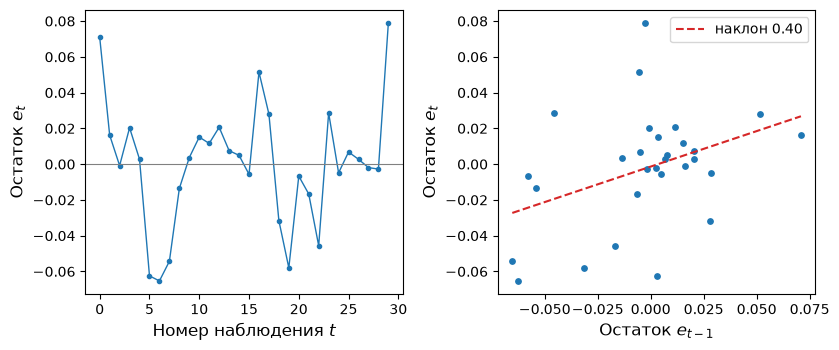
\includegraphics[keepaspectratio]{list11-diagnostic-acorr_files/figure-pdf/fig-icecream-resid-output-1.png}}

}

\caption{\label{fig-icecream-resid}ice cream equation: остатки модели во
времени и зависимость остатка от предыдущего}

\end{figure}%

\textbf{LM/BG-тест.} Проверьте модель на серийную корреляцию порядка 1.

{\def\LTcaptype{none} % do not increment counter
\begin{longtable}[]{@{}rrr@{}}
\toprule\noalign{}
LM-статистика & Степени свободы & P-значение \\
\midrule\noalign{}
\endhead
\bottomrule\noalign{}
\endlastfoot
4.237 & 1 & 0.040 \\
\end{longtable}
}

Вычислите критическое значение. \textbf{Ответ округлите до 2-х
десятичных знаков.}

\begin{tcolorbox}[enhanced jigsaw, arc=.35mm, bottomrule=.15mm, bottomtitle=1mm, breakable, colback=white, colbacktitle=quarto-callout-note-color!10!white, colframe=quarto-callout-note-color-frame, coltitle=black, left=2mm, leftrule=.75mm, opacityback=0, opacitybacktitle=0.6, rightrule=.15mm, title=\textcolor{quarto-callout-note-color}{\faInfo}\hspace{0.5em}{Критическое значение}, titlerule=0mm, toprule=.15mm, toptitle=1mm]

\(\chi^2_{crit} = 3.84\)

\end{tcolorbox}

Какой можно сделать вывод?

\begin{tcolorbox}[enhanced jigsaw, arc=.35mm, bottomrule=.15mm, bottomtitle=1mm, breakable, colback=white, colbacktitle=quarto-callout-tip-color!10!white, colframe=quarto-callout-tip-color-frame, coltitle=black, left=2mm, leftrule=.75mm, opacityback=0, opacitybacktitle=0.6, rightrule=.15mm, title=\textcolor{quarto-callout-tip-color}{\faLightbulb}\hspace{0.5em}{Вывод (BG-тест)}, titlerule=0mm, toprule=.15mm, toptitle=1mm]

\(LM = 4.237 > 3.84\), гипотеза \(H_0\) отвергается: серийная корреляция
порядка 1 есть.

\end{tcolorbox}

\subsection{consumption equation}\label{consumption-equation}

Для набора данных \texttt{Consumption} рассмотрим регрессию
\textbf{np.log(yd).diff() на np.log(ce).diff()}.

Переменные: \texttt{yd} --- располагаемый личный доход, \texttt{ce} ---
личные потребительские расходы (оба ряда --- в долларах 1986 г.).
Наблюдения --- квартальные, Канада, 1947--1996 гг.

Результаты оценивания:

{\def\LTcaptype{none} % do not increment counter
\begin{longtable}[]{@{}lr@{}}
\toprule\noalign{}
Переменная & Оценка \\
\midrule\noalign{}
\endhead
\bottomrule\noalign{}
\endlastfoot
Intercept & 0.006 \\
np.log(ce).diff() & 0.371 \\
\end{longtable}
}

Модель была подогнана по 199 наблюдениям.

\begin{tcolorbox}[enhanced jigsaw, arc=.35mm, bottomrule=.15mm, bottomtitle=1mm, breakable, colback=white, colbacktitle=quarto-callout-important-color!10!white, colframe=quarto-callout-important-color-frame, coltitle=black, left=2mm, leftrule=.75mm, opacityback=0, opacitybacktitle=0.6, rightrule=.15mm, title=\textcolor{quarto-callout-important-color}{\faExclamation}\hspace{0.5em}{Условия теста}, titlerule=0mm, toprule=.15mm, toptitle=1mm]

\begin{itemize}
\tightlist
\item
  уровень значимости: \textbf{1\%}
\item
  тест Дарбина--Уотсона: гипотеза \(H_0:\rho=0\) (автокорреляции первого
  порядка нет); границы \(d_L\), \(d_U\) --- для числа наблюдений
  \(n=199\) и числа регрессоров без константы \(k=1\)
\item
  тест Бройша--Годфри порядка 2, LM-статистика: гипотеза
  \(H_0:\rho_1=\rho_2=0\) (серийной корреляции порядка 2 нет);
  критическое значение --- по распределению \(\chi^2\) с числом степеней
  свободы 2
\end{itemize}

\end{tcolorbox}

\textbf{DW-тест.} Вычислите тестовую статистику. Найдите критические
значения \(d_L\), \(d_U\). Какой можно сделать вывод? \textbf{Статистику
округлите до 3-х десятичных знаков.}

{\def\LTcaptype{none} % do not increment counter
\begin{longtable}[]{@{}rrr@{}}
\toprule\noalign{}
DW & \(d_L\) & \(d_U\) \\
\midrule\noalign{}
\endhead
\bottomrule\noalign{}
\endlastfoot
2.382 & 1.663 & 1.683 \\
\end{longtable}
}

\begin{tcolorbox}[enhanced jigsaw, arc=.35mm, bottomrule=.15mm, bottomtitle=1mm, breakable, colback=white, colbacktitle=quarto-callout-tip-color!10!white, colframe=quarto-callout-tip-color-frame, coltitle=black, left=2mm, leftrule=.75mm, opacityback=0, opacitybacktitle=0.6, rightrule=.15mm, title=\textcolor{quarto-callout-tip-color}{\faLightbulb}\hspace{0.5em}{Вывод (DW-тест)}, titlerule=0mm, toprule=.15mm, toptitle=1mm]

\(DW = 2.382 > 4 - d_L = 2.337\), гипотеза \(H_0\) отвергается:
отрицательная автокорреляция первого порядка.

\end{tcolorbox}

\textbf{LM/BG-тест.} Проверьте модель на серийную корреляцию порядка 2.

{\def\LTcaptype{none} % do not increment counter
\begin{longtable}[]{@{}rrr@{}}
\toprule\noalign{}
LM-статистика & Степени свободы & P-значение \\
\midrule\noalign{}
\endhead
\bottomrule\noalign{}
\endlastfoot
8.913 & 2 & 0.012 \\
\end{longtable}
}

Вычислите критическое значение. \textbf{Ответ округлите до 2-х
десятичных знаков.}

\begin{tcolorbox}[enhanced jigsaw, arc=.35mm, bottomrule=.15mm, bottomtitle=1mm, breakable, colback=white, colbacktitle=quarto-callout-note-color!10!white, colframe=quarto-callout-note-color-frame, coltitle=black, left=2mm, leftrule=.75mm, opacityback=0, opacitybacktitle=0.6, rightrule=.15mm, title=\textcolor{quarto-callout-note-color}{\faInfo}\hspace{0.5em}{Критическое значение}, titlerule=0mm, toprule=.15mm, toptitle=1mm]

\(\chi^2_{crit} = 9.21\)

\end{tcolorbox}

Какой можно сделать вывод?

\begin{tcolorbox}[enhanced jigsaw, arc=.35mm, bottomrule=.15mm, bottomtitle=1mm, breakable, colback=white, colbacktitle=quarto-callout-tip-color!10!white, colframe=quarto-callout-tip-color-frame, coltitle=black, left=2mm, leftrule=.75mm, opacityback=0, opacitybacktitle=0.6, rightrule=.15mm, title=\textcolor{quarto-callout-tip-color}{\faLightbulb}\hspace{0.5em}{Вывод (BG-тест)}, titlerule=0mm, toprule=.15mm, toptitle=1mm]

\(LM = 8.913 < 9.21\), гипотеза \(H_0\) не отвергается: серийная
корреляция порядка 2 не выявлена. Выводы двух тестов расходятся: DW-тест
гипотезу об отсутствии автокорреляции отвергает, а BG-тест порядка 2 на
уровне 1\% не отвергает.

\end{tcolorbox}

\subsection{inflation equation \#1}\label{inflation-equation-1}

Для набора данных \texttt{Mishkin} рассмотрим регрессию
\textbf{pai3.diff() на tb3.diff(), np.log(cpi).diff()}.

Переменные: \texttt{pai3} --- трёхмесячный темп инфляции (в процентах
годовых), \texttt{tb3} --- ставка по трёхмесячным казначейским векселям
(в процентах годовых), \texttt{cpi} --- индекс потребительских цен
(среднее за 1982--1984 гг. равно 100). Наблюдения --- месячные, США,
1950--1990 гг.

Результаты оценивания:

{\def\LTcaptype{none} % do not increment counter
\begin{longtable}[]{@{}lr@{}}
\toprule\noalign{}
Переменная & Оценка \\
\midrule\noalign{}
\endhead
\bottomrule\noalign{}
\endlastfoot
Intercept & 0.162 \\
tb3.diff() & 0.081 \\
np.log(cpi).diff() & -44.823 \\
\end{longtable}
}

Модель была подогнана по 490 наблюдениям.

\begin{tcolorbox}[enhanced jigsaw, arc=.35mm, bottomrule=.15mm, bottomtitle=1mm, breakable, colback=white, colbacktitle=quarto-callout-important-color!10!white, colframe=quarto-callout-important-color-frame, coltitle=black, left=2mm, leftrule=.75mm, opacityback=0, opacitybacktitle=0.6, rightrule=.15mm, title=\textcolor{quarto-callout-important-color}{\faExclamation}\hspace{0.5em}{Условия теста}, titlerule=0mm, toprule=.15mm, toptitle=1mm]

\begin{itemize}
\tightlist
\item
  уровень значимости: \textbf{1\%}
\item
  тест Дарбина--Уотсона: гипотеза \(H_0:\rho=0\) (автокорреляции первого
  порядка нет); границы \(d_L\), \(d_U\) --- для числа наблюдений
  \(n=490\) и числа регрессоров без константы \(k=2\)
\item
  тест Бройша--Годфри порядка 2, LM-статистика: гипотеза
  \(H_0:\rho_1=\rho_2=0\) (серийной корреляции порядка 2 нет);
  критическое значение --- по распределению \(\chi^2\) с числом степеней
  свободы 2
\end{itemize}

\end{tcolorbox}

\textbf{DW-тест.} Вычислите тестовую статистику. Найдите критические
значения \(d_L\), \(d_U\). Какой можно сделать вывод? \textbf{Статистику
округлите до 3-х десятичных знаков.}

{\def\LTcaptype{none} % do not increment counter
\begin{longtable}[]{@{}rrr@{}}
\toprule\noalign{}
DW & \(d_L\) & \(d_U\) \\
\midrule\noalign{}
\endhead
\bottomrule\noalign{}
\endlastfoot
1.621 & 1.782 & 1.799 \\
\end{longtable}
}

\begin{tcolorbox}[enhanced jigsaw, arc=.35mm, bottomrule=.15mm, bottomtitle=1mm, breakable, colback=white, colbacktitle=quarto-callout-tip-color!10!white, colframe=quarto-callout-tip-color-frame, coltitle=black, left=2mm, leftrule=.75mm, opacityback=0, opacitybacktitle=0.6, rightrule=.15mm, title=\textcolor{quarto-callout-tip-color}{\faLightbulb}\hspace{0.5em}{Вывод (DW-тест)}, titlerule=0mm, toprule=.15mm, toptitle=1mm]

\(DW = 1.621 < d_L = 1.782\), гипотеза \(H_0\) отвергается:
положительная автокорреляция первого порядка.

\end{tcolorbox}

\textbf{LM/BG-тест.} Проверьте модель на серийную корреляцию порядка 2.

{\def\LTcaptype{none} % do not increment counter
\begin{longtable}[]{@{}rrr@{}}
\toprule\noalign{}
LM-статистика & Степени свободы & P-значение \\
\midrule\noalign{}
\endhead
\bottomrule\noalign{}
\endlastfoot
17.200 & 2 & \textless0.001 \\
\end{longtable}
}

Вычислите критическое значение. \textbf{Ответ округлите до 2-х
десятичных знаков.}

\begin{tcolorbox}[enhanced jigsaw, arc=.35mm, bottomrule=.15mm, bottomtitle=1mm, breakable, colback=white, colbacktitle=quarto-callout-note-color!10!white, colframe=quarto-callout-note-color-frame, coltitle=black, left=2mm, leftrule=.75mm, opacityback=0, opacitybacktitle=0.6, rightrule=.15mm, title=\textcolor{quarto-callout-note-color}{\faInfo}\hspace{0.5em}{Критическое значение}, titlerule=0mm, toprule=.15mm, toptitle=1mm]

\(\chi^2_{crit} = 9.21\)

\end{tcolorbox}

Какой можно сделать вывод?

\begin{tcolorbox}[enhanced jigsaw, arc=.35mm, bottomrule=.15mm, bottomtitle=1mm, breakable, colback=white, colbacktitle=quarto-callout-tip-color!10!white, colframe=quarto-callout-tip-color-frame, coltitle=black, left=2mm, leftrule=.75mm, opacityback=0, opacitybacktitle=0.6, rightrule=.15mm, title=\textcolor{quarto-callout-tip-color}{\faLightbulb}\hspace{0.5em}{Вывод (BG-тест)}, titlerule=0mm, toprule=.15mm, toptitle=1mm]

\(LM = 17.200 > 9.21\), гипотеза \(H_0\) отвергается: серийная
корреляция порядка 2 есть.

\end{tcolorbox}

\subsection{inflation equation \#2}\label{inflation-equation-2}

Для набора данных \texttt{Tbrate} рассмотрим регрессию \textbf{pi.diff()
на y.diff(), r.diff()}.

Переменные: \texttt{pi} --- темп инфляции, \texttt{y} --- логарифм
реального ВВП, \texttt{r} --- ставка по 91-дневным казначейским
векселям. Наблюдения --- квартальные, Канада, 1950--1996 гг.

Результаты оценивания:

{\def\LTcaptype{none} % do not increment counter
\begin{longtable}[]{@{}lr@{}}
\toprule\noalign{}
Переменная & Оценка \\
\midrule\noalign{}
\endhead
\bottomrule\noalign{}
\endlastfoot
Intercept & 0.091 \\
y.diff() & -9.130 \\
r.diff() & 0.311 \\
\end{longtable}
}

Модель была подогнана по 187 наблюдениям.

\begin{tcolorbox}[enhanced jigsaw, arc=.35mm, bottomrule=.15mm, bottomtitle=1mm, breakable, colback=white, colbacktitle=quarto-callout-important-color!10!white, colframe=quarto-callout-important-color-frame, coltitle=black, left=2mm, leftrule=.75mm, opacityback=0, opacitybacktitle=0.6, rightrule=.15mm, title=\textcolor{quarto-callout-important-color}{\faExclamation}\hspace{0.5em}{Условия теста}, titlerule=0mm, toprule=.15mm, toptitle=1mm]

\begin{itemize}
\tightlist
\item
  уровень значимости: \textbf{5\%}
\item
  тест Дарбина--Уотсона: гипотеза \(H_0:\rho=0\) (автокорреляции первого
  порядка нет); границы \(d_L\), \(d_U\) --- для числа наблюдений
  \(n=187\) и числа регрессоров без константы \(k=2\)
\item
  тест Бройша--Годфри порядка 1, LM-статистика: гипотеза
  \(H_0:\rho_1=0\) (серийной корреляции порядка 1 нет); критическое
  значение --- по распределению \(\chi^2\) с числом степеней свободы 1
\end{itemize}

\end{tcolorbox}

\textbf{DW-тест.} Вычислите тестовую статистику. Найдите критические
значения \(d_L\), \(d_U\). Какой можно сделать вывод? \textbf{Статистику
округлите до 3-х десятичных знаков.}

{\def\LTcaptype{none} % do not increment counter
\begin{longtable}[]{@{}rrr@{}}
\toprule\noalign{}
DW & \(d_L\) & \(d_U\) \\
\midrule\noalign{}
\endhead
\bottomrule\noalign{}
\endlastfoot
2.459 & 1.739 & 1.782 \\
\end{longtable}
}

\begin{tcolorbox}[enhanced jigsaw, arc=.35mm, bottomrule=.15mm, bottomtitle=1mm, breakable, colback=white, colbacktitle=quarto-callout-tip-color!10!white, colframe=quarto-callout-tip-color-frame, coltitle=black, left=2mm, leftrule=.75mm, opacityback=0, opacitybacktitle=0.6, rightrule=.15mm, title=\textcolor{quarto-callout-tip-color}{\faLightbulb}\hspace{0.5em}{Вывод (DW-тест)}, titlerule=0mm, toprule=.15mm, toptitle=1mm]

\(DW = 2.459 > 4 - d_L = 2.261\), гипотеза \(H_0\) отвергается:
отрицательная автокорреляция первого порядка.

\end{tcolorbox}

\textbf{LM/BG-тест.} Проверьте модель на серийную корреляцию порядка 1.

{\def\LTcaptype{none} % do not increment counter
\begin{longtable}[]{@{}rrr@{}}
\toprule\noalign{}
LM-статистика & Степени свободы & P-значение \\
\midrule\noalign{}
\endhead
\bottomrule\noalign{}
\endlastfoot
10.683 & 1 & 0.001 \\
\end{longtable}
}

Вычислите критическое значение. \textbf{Ответ округлите до 2-х
десятичных знаков.}

\begin{tcolorbox}[enhanced jigsaw, arc=.35mm, bottomrule=.15mm, bottomtitle=1mm, breakable, colback=white, colbacktitle=quarto-callout-note-color!10!white, colframe=quarto-callout-note-color-frame, coltitle=black, left=2mm, leftrule=.75mm, opacityback=0, opacitybacktitle=0.6, rightrule=.15mm, title=\textcolor{quarto-callout-note-color}{\faInfo}\hspace{0.5em}{Критическое значение}, titlerule=0mm, toprule=.15mm, toptitle=1mm]

\(\chi^2_{crit} = 3.84\)

\end{tcolorbox}

Какой можно сделать вывод?

\begin{tcolorbox}[enhanced jigsaw, arc=.35mm, bottomrule=.15mm, bottomtitle=1mm, breakable, colback=white, colbacktitle=quarto-callout-tip-color!10!white, colframe=quarto-callout-tip-color-frame, coltitle=black, left=2mm, leftrule=.75mm, opacityback=0, opacitybacktitle=0.6, rightrule=.15mm, title=\textcolor{quarto-callout-tip-color}{\faLightbulb}\hspace{0.5em}{Вывод (BG-тест)}, titlerule=0mm, toprule=.15mm, toptitle=1mm]

\(LM = 10.683 > 3.84\), гипотеза \(H_0\) отвергается: серийная
корреляция порядка 1 есть.

\end{tcolorbox}

\subsection{inflation equation \#3}\label{inflation-equation-3}

Для набора данных \texttt{MoneyUS} рассмотрим регрессию

\texttt{infl.diff()\ \textasciitilde{}\ y.diff()\ +\ tbr.diff()\ +\ cpr.diff()\ +\ m.diff()}

Переменные: \texttt{infl} --- квартальный темп инфляции (в процентах
годовых), \texttt{y} --- логарифм реального ВВП, \texttt{tbr} --- ставка
по казначейским векселям, \texttt{cpr} --- ставка по коммерческим
бумагам (в процентах годовых), \texttt{m} --- логарифм реальной денежной
массы M1. Наблюдения --- квартальные, США, 1954--1994 гг.

Результаты оценивания (оценки в этой задаче малы по величине, поэтому
приведены с 5 десятичными знаками):

{\def\LTcaptype{none} % do not increment counter
\begin{longtable}[]{@{}lr@{}}
\toprule\noalign{}
Переменная & Оценка \\
\midrule\noalign{}
\endhead
\bottomrule\noalign{}
\endlastfoot
Intercept & -0.00013 \\
y.diff() & -0.00241 \\
tbr.diff() & 0.00017 \\
cpr.diff() & 0.40710 \\
m.diff() & -0.00124 \\
\end{longtable}
}

Модель была подогнана по 163 наблюдениям.

\begin{tcolorbox}[enhanced jigsaw, arc=.35mm, bottomrule=.15mm, bottomtitle=1mm, breakable, colback=white, colbacktitle=quarto-callout-important-color!10!white, colframe=quarto-callout-important-color-frame, coltitle=black, left=2mm, leftrule=.75mm, opacityback=0, opacitybacktitle=0.6, rightrule=.15mm, title=\textcolor{quarto-callout-important-color}{\faExclamation}\hspace{0.5em}{Условия теста}, titlerule=0mm, toprule=.15mm, toptitle=1mm]

\begin{itemize}
\tightlist
\item
  уровень значимости: \textbf{1\%}
\item
  тест Дарбина--Уотсона: гипотеза \(H_0:\rho=0\) (автокорреляции первого
  порядка нет); границы \(d_L\), \(d_U\) --- для числа наблюдений
  \(n=163\) и числа регрессоров без константы \(k=4\)
\item
  тест Бройша--Годфри порядка 2, LM-статистика: гипотеза
  \(H_0:\rho_1=\rho_2=0\) (серийной корреляции порядка 2 нет);
  критическое значение --- по распределению \(\chi^2\) с числом степеней
  свободы 2
\end{itemize}

\end{tcolorbox}

\textbf{DW-тест.} Вычислите тестовую статистику. Найдите критические
значения \(d_L\), \(d_U\). Какой можно сделать вывод? \textbf{Статистику
округлите до 3-х десятичных знаков.}

{\def\LTcaptype{none} % do not increment counter
\begin{longtable}[]{@{}rrr@{}}
\toprule\noalign{}
DW & \(d_L\) & \(d_U\) \\
\midrule\noalign{}
\endhead
\bottomrule\noalign{}
\endlastfoot
0.834 & 1.590 & 1.689 \\
\end{longtable}
}

\begin{tcolorbox}[enhanced jigsaw, arc=.35mm, bottomrule=.15mm, bottomtitle=1mm, breakable, colback=white, colbacktitle=quarto-callout-tip-color!10!white, colframe=quarto-callout-tip-color-frame, coltitle=black, left=2mm, leftrule=.75mm, opacityback=0, opacitybacktitle=0.6, rightrule=.15mm, title=\textcolor{quarto-callout-tip-color}{\faLightbulb}\hspace{0.5em}{Вывод (DW-тест)}, titlerule=0mm, toprule=.15mm, toptitle=1mm]

\(DW = 0.834 < d_L = 1.590\), гипотеза \(H_0\) отвергается:
положительная автокорреляция первого порядка.

\end{tcolorbox}

Остатки модели показывает Рисунок~\ref{fig-moneyus-resid}: соседние
остатки связаны положительно.

\begin{figure}

\centering{

\pandocbounded{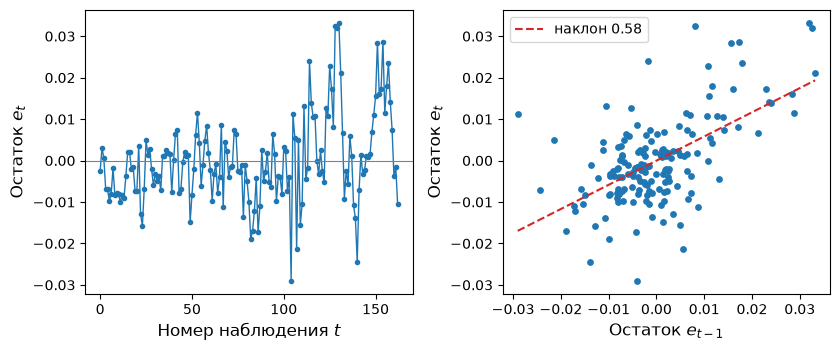
\includegraphics[keepaspectratio]{list11-diagnostic-acorr_files/figure-pdf/fig-moneyus-resid-output-1.png}}

}

\caption{\label{fig-moneyus-resid}inflation equation \#3: остатки модели
во времени и зависимость остатка от предыдущего}

\end{figure}%

\textbf{LM/BG-тест.} Проверьте модель на серийную корреляцию порядка 2.

{\def\LTcaptype{none} % do not increment counter
\begin{longtable}[]{@{}rrr@{}}
\toprule\noalign{}
LM-статистика & Степени свободы & P-значение \\
\midrule\noalign{}
\endhead
\bottomrule\noalign{}
\endlastfoot
61.893 & 2 & \textless0.001 \\
\end{longtable}
}

Вычислите критическое значение. \textbf{Ответ округлите до 2-х
десятичных знаков.}

\begin{tcolorbox}[enhanced jigsaw, arc=.35mm, bottomrule=.15mm, bottomtitle=1mm, breakable, colback=white, colbacktitle=quarto-callout-note-color!10!white, colframe=quarto-callout-note-color-frame, coltitle=black, left=2mm, leftrule=.75mm, opacityback=0, opacitybacktitle=0.6, rightrule=.15mm, title=\textcolor{quarto-callout-note-color}{\faInfo}\hspace{0.5em}{Критическое значение}, titlerule=0mm, toprule=.15mm, toptitle=1mm]

\(\chi^2_{crit} = 9.21\)

\end{tcolorbox}

Какой можно сделать вывод?

\begin{tcolorbox}[enhanced jigsaw, arc=.35mm, bottomrule=.15mm, bottomtitle=1mm, breakable, colback=white, colbacktitle=quarto-callout-tip-color!10!white, colframe=quarto-callout-tip-color-frame, coltitle=black, left=2mm, leftrule=.75mm, opacityback=0, opacitybacktitle=0.6, rightrule=.15mm, title=\textcolor{quarto-callout-tip-color}{\faLightbulb}\hspace{0.5em}{Вывод (BG-тест)}, titlerule=0mm, toprule=.15mm, toptitle=1mm]

\(LM = 61.893 > 9.21\), гипотеза \(H_0\) отвергается: серийная
корреляция порядка 2 есть.

\end{tcolorbox}

\subsection{unemployment equation}\label{unemployment-equation}

Для набора данных \texttt{Macrodat} рассмотрим регрессию

\begin{Shaded}
\begin{Highlighting}[]
\NormalTok{lhur.diff() }\OperatorTok{\textasciitilde{}}\NormalTok{ np.log(punew).diff() }\OperatorTok{+}\NormalTok{ fyff.diff() }\OperatorTok{+}\NormalTok{ fygm3.diff() }\OperatorTok{+}
\NormalTok{              fygt1.diff() }\OperatorTok{+}\NormalTok{ np.log(gdpjp).diff()}
\end{Highlighting}
\end{Shaded}

Переменные: \texttt{lhur} --- уровень безработицы (в процентах),
\texttt{punew} --- индекс потребительских цен, \texttt{fyff} --- ставка
по федеральным фондам, \texttt{fygm3} и \texttt{fygt1} --- ставки по
трёхмесячным и годовым казначейским бумагам, \texttt{gdpjp} --- реальный
ВВП Японии. Наблюдения --- квартальные, США, 1959--2000 гг.

Результаты оценивания:

{\def\LTcaptype{none} % do not increment counter
\begin{longtable}[]{@{}lr@{}}
\toprule\noalign{}
Переменная & Оценка \\
\midrule\noalign{}
\endhead
\bottomrule\noalign{}
\endlastfoot
Intercept & -0.141 \\
np.log(punew).diff() & 12.720 \\
fyff.diff() & -0.115 \\
fygm3.diff() & 0.168 \\
fygt1.diff() & -0.166 \\
np.log(gdpjp).diff() & -0.399 \\
\end{longtable}
}

Модель была подогнана по 161 наблюдению.

В наборе 168 кварталов; последние 6 значений \texttt{gdpjp} пропущены,
ещё одно наблюдение теряется при взятии разности.

\begin{tcolorbox}[enhanced jigsaw, arc=.35mm, bottomrule=.15mm, bottomtitle=1mm, breakable, colback=white, colbacktitle=quarto-callout-important-color!10!white, colframe=quarto-callout-important-color-frame, coltitle=black, left=2mm, leftrule=.75mm, opacityback=0, opacitybacktitle=0.6, rightrule=.15mm, title=\textcolor{quarto-callout-important-color}{\faExclamation}\hspace{0.5em}{Условия теста}, titlerule=0mm, toprule=.15mm, toptitle=1mm]

\begin{itemize}
\tightlist
\item
  уровень значимости: \textbf{1\%}
\item
  тест Дарбина--Уотсона: гипотеза \(H_0:\rho=0\) (автокорреляции первого
  порядка нет); границы \(d_L\), \(d_U\) --- для числа наблюдений
  \(n=161\) и числа регрессоров без константы \(k=5\)
\item
  тест Бройша--Годфри порядка 2, LM-статистика: гипотеза
  \(H_0:\rho_1=\rho_2=0\) (серийной корреляции порядка 2 нет);
  критическое значение --- по распределению \(\chi^2\) с числом степеней
  свободы 2
\end{itemize}

\end{tcolorbox}

\textbf{DW-тест.} Вычислите тестовую статистику. Найдите критические
значения \(d_L\), \(d_U\). Какой можно сделать вывод? \textbf{Статистику
округлите до 3-х десятичных знаков.}

{\def\LTcaptype{none} % do not increment counter
\begin{longtable}[]{@{}rrr@{}}
\toprule\noalign{}
DW & \(d_L\) & \(d_U\) \\
\midrule\noalign{}
\endhead
\bottomrule\noalign{}
\endlastfoot
1.063 & 1.574 & 1.701 \\
\end{longtable}
}

\begin{tcolorbox}[enhanced jigsaw, arc=.35mm, bottomrule=.15mm, bottomtitle=1mm, breakable, colback=white, colbacktitle=quarto-callout-tip-color!10!white, colframe=quarto-callout-tip-color-frame, coltitle=black, left=2mm, leftrule=.75mm, opacityback=0, opacitybacktitle=0.6, rightrule=.15mm, title=\textcolor{quarto-callout-tip-color}{\faLightbulb}\hspace{0.5em}{Вывод (DW-тест)}, titlerule=0mm, toprule=.15mm, toptitle=1mm]

\(DW = 1.063 < d_L = 1.574\), гипотеза \(H_0\) отвергается:
положительная автокорреляция первого порядка.

\end{tcolorbox}

\textbf{LM/BG-тест.} Проверьте модель на серийную корреляцию порядка 2.

{\def\LTcaptype{none} % do not increment counter
\begin{longtable}[]{@{}rrr@{}}
\toprule\noalign{}
LM-статистика & Степени свободы & P-значение \\
\midrule\noalign{}
\endhead
\bottomrule\noalign{}
\endlastfoot
35.658 & 2 & \textless0.001 \\
\end{longtable}
}

Вычислите критическое значение. \textbf{Ответ округлите до 2-х
десятичных знаков.}

\begin{tcolorbox}[enhanced jigsaw, arc=.35mm, bottomrule=.15mm, bottomtitle=1mm, breakable, colback=white, colbacktitle=quarto-callout-note-color!10!white, colframe=quarto-callout-note-color-frame, coltitle=black, left=2mm, leftrule=.75mm, opacityback=0, opacitybacktitle=0.6, rightrule=.15mm, title=\textcolor{quarto-callout-note-color}{\faInfo}\hspace{0.5em}{Критическое значение}, titlerule=0mm, toprule=.15mm, toptitle=1mm]

\(\chi^2_{crit} = 9.21\)

\end{tcolorbox}

Какой можно сделать вывод?

\begin{tcolorbox}[enhanced jigsaw, arc=.35mm, bottomrule=.15mm, bottomtitle=1mm, breakable, colback=white, colbacktitle=quarto-callout-tip-color!10!white, colframe=quarto-callout-tip-color-frame, coltitle=black, left=2mm, leftrule=.75mm, opacityback=0, opacitybacktitle=0.6, rightrule=.15mm, title=\textcolor{quarto-callout-tip-color}{\faLightbulb}\hspace{0.5em}{Вывод (BG-тест)}, titlerule=0mm, toprule=.15mm, toptitle=1mm]

\(LM = 35.658 > 9.21\), гипотеза \(H_0\) отвергается: серийная
корреляция порядка 2 есть.

\end{tcolorbox}

\section{Робастный t-тест
(HAC-ошибки)}\label{ux440ux43eux431ux430ux441ux442ux43dux44bux439-t-ux442ux435ux441ux442-hac-ux43eux448ux438ux431ux43aux438}

\subsection{ice cream equation}\label{ice-cream-equation-1}

Для набора данных \texttt{Icecream} рассмотрим регрессию \textbf{cons на
income, price, temp}.

\begin{tcolorbox}[enhanced jigsaw, arc=.35mm, bottomrule=.15mm, bottomtitle=1mm, breakable, colback=white, colbacktitle=quarto-callout-important-color!10!white, colframe=quarto-callout-important-color-frame, coltitle=black, left=2mm, leftrule=.75mm, opacityback=0, opacitybacktitle=0.6, rightrule=.15mm, title=\textcolor{quarto-callout-important-color}{\faExclamation}\hspace{0.5em}{Условия теста}, titlerule=0mm, toprule=.15mm, toptitle=1mm]

\begin{itemize}
\tightlist
\item
  уровень значимости: \textbf{1\%}
\item
  стандартные ошибки: \textbf{неробастные и робастные HAC (Ньюи--Уэст,
  ядро Бартлетта), \texttt{maxlags\ =\ 3}}
\item
  гипотеза: \(H_0:\beta_j=0\) для каждого коэффициента, альтернатива
  двусторонняя
\item
  число лагов: \(L=\lfloor 4\,(n/100)^{2/9}\rfloor = 3\) при \(n=30\)
\end{itemize}

\end{tcolorbox}

\textbf{Результаты \(t\)-теста для коэффициентов (неробастные
стандартные ошибки):}

{\def\LTcaptype{none} % do not increment counter
\begin{longtable}[]{@{}lrrrrl@{}}
\toprule\noalign{}
& Coef. & Std.Err. & t-value & p-value & Signif. \\
\midrule\noalign{}
\endhead
\bottomrule\noalign{}
\endlastfoot
Intercept & 0.197 & 0.270 & 0.730 & 0.472 & \\
income & 0.003 & 0.001 & 2.824 & 0.009 & *** \\
price & -1.044 & 0.834 & -1.252 & 0.222 & \\
temp & 0.003 & 0.000446 & 7.762 & \textless0.001 & *** \\
\end{longtable}
}

\emph{Signif. codes:} \texttt{***} \(p<0.01\), \texttt{**} \(p<0.05\),
\texttt{*} \(p<0.1\)

Какие коэффициенты значимы?

\begin{tcolorbox}[enhanced jigsaw, arc=.35mm, bottomrule=.15mm, bottomtitle=1mm, breakable, colback=white, colbacktitle=quarto-callout-note-color!10!white, colframe=quarto-callout-note-color-frame, coltitle=black, left=2mm, leftrule=.75mm, opacityback=0, opacitybacktitle=0.6, rightrule=.15mm, title=\textcolor{quarto-callout-note-color}{\faInfo}\hspace{0.5em}{Коэффициенты, значимые на уровне 1\% (по неробастным стандартным
ошибкам)}, titlerule=0mm, toprule=.15mm, toptitle=1mm]

\texttt{income}, \texttt{temp}

\end{tcolorbox}

\textbf{Результаты \(t\)-теста для коэффициентов (робастные стандартные
ошибки, HAC):}

{\def\LTcaptype{none} % do not increment counter
\begin{longtable}[]{@{}lrrrrl@{}}
\toprule\noalign{}
& Coef. & Std.Err. & t-value & p-value & Signif. \\
\midrule\noalign{}
\endhead
\bottomrule\noalign{}
\endlastfoot
Intercept & 0.197 & 0.314 & 0.627 & 0.536 & \\
income & 0.003 & 0.001 & 2.676 & 0.013 & ** \\
price & -1.044 & 0.910 & -1.148 & 0.261 & \\
temp & 0.003 & 0.000373 & 9.282 & \textless0.001 & *** \\
\end{longtable}
}

\emph{Signif. codes:} \texttt{***} \(p<0.01\), \texttt{**} \(p<0.05\),
\texttt{*} \(p<0.1\)

Какие коэффициенты значимы?

\begin{tcolorbox}[enhanced jigsaw, arc=.35mm, bottomrule=.15mm, bottomtitle=1mm, breakable, colback=white, colbacktitle=quarto-callout-note-color!10!white, colframe=quarto-callout-note-color-frame, coltitle=black, left=2mm, leftrule=.75mm, opacityback=0, opacitybacktitle=0.6, rightrule=.15mm, title=\textcolor{quarto-callout-note-color}{\faInfo}\hspace{0.5em}{Коэффициенты, значимые на уровне 1\% (по робастным стандартным ошибкам
HAC)}, titlerule=0mm, toprule=.15mm, toptitle=1mm]

\texttt{temp}

\end{tcolorbox}

\subsection{consumption equation}\label{consumption-equation-1}

Для набора данных \texttt{Consumption} рассмотрим регрессию
\textbf{np.log(yd).diff() на np.log(ce).diff()}.

\begin{tcolorbox}[enhanced jigsaw, arc=.35mm, bottomrule=.15mm, bottomtitle=1mm, breakable, colback=white, colbacktitle=quarto-callout-important-color!10!white, colframe=quarto-callout-important-color-frame, coltitle=black, left=2mm, leftrule=.75mm, opacityback=0, opacitybacktitle=0.6, rightrule=.15mm, title=\textcolor{quarto-callout-important-color}{\faExclamation}\hspace{0.5em}{Условия теста}, titlerule=0mm, toprule=.15mm, toptitle=1mm]

\begin{itemize}
\tightlist
\item
  уровень значимости: \textbf{1\%}
\item
  стандартные ошибки: \textbf{неробастные и робастные HAC (Ньюи--Уэст,
  ядро Бартлетта), \texttt{maxlags\ =\ 4}}
\item
  гипотеза: \(H_0:\beta_j=0\) для каждого коэффициента, альтернатива
  двусторонняя
\item
  число лагов: \(L=\lfloor 4\,(n/100)^{2/9}\rfloor = 4\) при \(n=199\)
\end{itemize}

\end{tcolorbox}

\textbf{Результаты \(t\)-теста для коэффициентов (неробастные
стандартные ошибки):}

{\def\LTcaptype{none} % do not increment counter
\begin{longtable}[]{@{}
  >{\raggedright\arraybackslash}p{(\linewidth - 10\tabcolsep) * \real{0.2603}}
  >{\raggedleft\arraybackslash}p{(\linewidth - 10\tabcolsep) * \real{0.1233}}
  >{\raggedleft\arraybackslash}p{(\linewidth - 10\tabcolsep) * \real{0.1644}}
  >{\raggedleft\arraybackslash}p{(\linewidth - 10\tabcolsep) * \real{0.1507}}
  >{\raggedleft\arraybackslash}p{(\linewidth - 10\tabcolsep) * \real{0.1507}}
  >{\raggedright\arraybackslash}p{(\linewidth - 10\tabcolsep) * \real{0.1507}}@{}}
\toprule\noalign{}
\begin{minipage}[b]{\linewidth}\raggedright
\end{minipage} & \begin{minipage}[b]{\linewidth}\raggedleft
Coef.
\end{minipage} & \begin{minipage}[b]{\linewidth}\raggedleft
Std.Err.
\end{minipage} & \begin{minipage}[b]{\linewidth}\raggedleft
t-value
\end{minipage} & \begin{minipage}[b]{\linewidth}\raggedleft
p-value
\end{minipage} & \begin{minipage}[b]{\linewidth}\raggedright
Signif.
\end{minipage} \\
\midrule\noalign{}
\endhead
\bottomrule\noalign{}
\endlastfoot
Intercept & 0.006 & 0.001 & 5.252 & \textless0.001 & \\
np.log(ce).diff() & 0.371 & 0.068 & 5.483 & \textless0.001 & *** \\
\end{longtable}
}

\emph{Signif. codes:} \texttt{***} \(p<0.01\), \texttt{**} \(p<0.05\),
\texttt{*} \(p<0.1\)

Какие коэффициенты значимы?

\begin{tcolorbox}[enhanced jigsaw, arc=.35mm, bottomrule=.15mm, bottomtitle=1mm, breakable, colback=white, colbacktitle=quarto-callout-note-color!10!white, colframe=quarto-callout-note-color-frame, coltitle=black, left=2mm, leftrule=.75mm, opacityback=0, opacitybacktitle=0.6, rightrule=.15mm, title=\textcolor{quarto-callout-note-color}{\faInfo}\hspace{0.5em}{Коэффициенты, значимые на уровне 1\% (по неробастным стандартным
ошибкам)}, titlerule=0mm, toprule=.15mm, toptitle=1mm]

\texttt{np.log(ce).diff()}

\end{tcolorbox}

\textbf{Результаты \(t\)-теста для коэффициентов (робастные стандартные
ошибки, HAC):}

{\def\LTcaptype{none} % do not increment counter
\begin{longtable}[]{@{}
  >{\raggedright\arraybackslash}p{(\linewidth - 10\tabcolsep) * \real{0.2603}}
  >{\raggedleft\arraybackslash}p{(\linewidth - 10\tabcolsep) * \real{0.1233}}
  >{\raggedleft\arraybackslash}p{(\linewidth - 10\tabcolsep) * \real{0.1644}}
  >{\raggedleft\arraybackslash}p{(\linewidth - 10\tabcolsep) * \real{0.1507}}
  >{\raggedleft\arraybackslash}p{(\linewidth - 10\tabcolsep) * \real{0.1507}}
  >{\raggedright\arraybackslash}p{(\linewidth - 10\tabcolsep) * \real{0.1507}}@{}}
\toprule\noalign{}
\begin{minipage}[b]{\linewidth}\raggedright
\end{minipage} & \begin{minipage}[b]{\linewidth}\raggedleft
Coef.
\end{minipage} & \begin{minipage}[b]{\linewidth}\raggedleft
Std.Err.
\end{minipage} & \begin{minipage}[b]{\linewidth}\raggedleft
t-value
\end{minipage} & \begin{minipage}[b]{\linewidth}\raggedleft
p-value
\end{minipage} & \begin{minipage}[b]{\linewidth}\raggedright
Signif.
\end{minipage} \\
\midrule\noalign{}
\endhead
\bottomrule\noalign{}
\endlastfoot
Intercept & 0.006 & 0.001 & 4.943 & \textless0.001 & \\
np.log(ce).diff() & 0.371 & 0.079 & 4.668 & \textless0.001 & *** \\
\end{longtable}
}

\emph{Signif. codes:} \texttt{***} \(p<0.01\), \texttt{**} \(p<0.05\),
\texttt{*} \(p<0.1\)

Какие коэффициенты значимы?

\begin{tcolorbox}[enhanced jigsaw, arc=.35mm, bottomrule=.15mm, bottomtitle=1mm, breakable, colback=white, colbacktitle=quarto-callout-note-color!10!white, colframe=quarto-callout-note-color-frame, coltitle=black, left=2mm, leftrule=.75mm, opacityback=0, opacitybacktitle=0.6, rightrule=.15mm, title=\textcolor{quarto-callout-note-color}{\faInfo}\hspace{0.5em}{Коэффициенты, значимые на уровне 1\% (по робастным стандартным ошибкам
HAC)}, titlerule=0mm, toprule=.15mm, toptitle=1mm]

\texttt{np.log(ce).diff()}

\end{tcolorbox}

\subsection{inflation equation \#1}\label{inflation-equation-1-1}

Для набора данных \texttt{Mishkin} рассмотрим регрессию
\textbf{pai3.diff() на tb3.diff(), np.log(cpi).diff()}.

\begin{tcolorbox}[enhanced jigsaw, arc=.35mm, bottomrule=.15mm, bottomtitle=1mm, breakable, colback=white, colbacktitle=quarto-callout-important-color!10!white, colframe=quarto-callout-important-color-frame, coltitle=black, left=2mm, leftrule=.75mm, opacityback=0, opacitybacktitle=0.6, rightrule=.15mm, title=\textcolor{quarto-callout-important-color}{\faExclamation}\hspace{0.5em}{Условия теста}, titlerule=0mm, toprule=.15mm, toptitle=1mm]

\begin{itemize}
\tightlist
\item
  уровень значимости: \textbf{1\%}
\item
  стандартные ошибки: \textbf{неробастные и робастные HAC (Ньюи--Уэст,
  ядро Бартлетта), \texttt{maxlags\ =\ 5}}
\item
  гипотеза: \(H_0:\beta_j=0\) для каждого коэффициента, альтернатива
  двусторонняя
\item
  число лагов: \(L=\lfloor 4\,(n/100)^{2/9}\rfloor = 5\) при \(n=490\)
\end{itemize}

\end{tcolorbox}

\textbf{Результаты \(t\)-теста для коэффициентов (неробастные
стандартные ошибки):}

{\def\LTcaptype{none} % do not increment counter
\begin{longtable}[]{@{}
  >{\raggedright\arraybackslash}p{(\linewidth - 10\tabcolsep) * \real{0.2703}}
  >{\raggedleft\arraybackslash}p{(\linewidth - 10\tabcolsep) * \real{0.1216}}
  >{\raggedleft\arraybackslash}p{(\linewidth - 10\tabcolsep) * \real{0.1622}}
  >{\raggedleft\arraybackslash}p{(\linewidth - 10\tabcolsep) * \real{0.1486}}
  >{\raggedleft\arraybackslash}p{(\linewidth - 10\tabcolsep) * \real{0.1486}}
  >{\raggedright\arraybackslash}p{(\linewidth - 10\tabcolsep) * \real{0.1486}}@{}}
\toprule\noalign{}
\begin{minipage}[b]{\linewidth}\raggedright
\end{minipage} & \begin{minipage}[b]{\linewidth}\raggedleft
Coef.
\end{minipage} & \begin{minipage}[b]{\linewidth}\raggedleft
Std.Err.
\end{minipage} & \begin{minipage}[b]{\linewidth}\raggedleft
t-value
\end{minipage} & \begin{minipage}[b]{\linewidth}\raggedleft
p-value
\end{minipage} & \begin{minipage}[b]{\linewidth}\raggedright
Signif.
\end{minipage} \\
\midrule\noalign{}
\endhead
\bottomrule\noalign{}
\endlastfoot
Intercept & 0.162 & 0.087 & 1.860 & 0.063 & \\
tb3.diff() & 0.081 & 0.112 & 0.726 & 0.468 & \\
np.log(cpi).diff() & -44.823 & 17.130 & -2.617 & 0.009 & *** \\
\end{longtable}
}

\emph{Signif. codes:} \texttt{***} \(p<0.01\), \texttt{**} \(p<0.05\),
\texttt{*} \(p<0.1\)

Какие коэффициенты значимы?

\begin{tcolorbox}[enhanced jigsaw, arc=.35mm, bottomrule=.15mm, bottomtitle=1mm, breakable, colback=white, colbacktitle=quarto-callout-note-color!10!white, colframe=quarto-callout-note-color-frame, coltitle=black, left=2mm, leftrule=.75mm, opacityback=0, opacitybacktitle=0.6, rightrule=.15mm, title=\textcolor{quarto-callout-note-color}{\faInfo}\hspace{0.5em}{Коэффициенты, значимые на уровне 1\% (по неробастным стандартным
ошибкам)}, titlerule=0mm, toprule=.15mm, toptitle=1mm]

\texttt{np.log(cpi).diff()}

\end{tcolorbox}

\textbf{Результаты \(t\)-теста для коэффициентов (робастные стандартные
ошибки, HAC):}

{\def\LTcaptype{none} % do not increment counter
\begin{longtable}[]{@{}
  >{\raggedright\arraybackslash}p{(\linewidth - 10\tabcolsep) * \real{0.2703}}
  >{\raggedleft\arraybackslash}p{(\linewidth - 10\tabcolsep) * \real{0.1216}}
  >{\raggedleft\arraybackslash}p{(\linewidth - 10\tabcolsep) * \real{0.1622}}
  >{\raggedleft\arraybackslash}p{(\linewidth - 10\tabcolsep) * \real{0.1486}}
  >{\raggedleft\arraybackslash}p{(\linewidth - 10\tabcolsep) * \real{0.1486}}
  >{\raggedright\arraybackslash}p{(\linewidth - 10\tabcolsep) * \real{0.1486}}@{}}
\toprule\noalign{}
\begin{minipage}[b]{\linewidth}\raggedright
\end{minipage} & \begin{minipage}[b]{\linewidth}\raggedleft
Coef.
\end{minipage} & \begin{minipage}[b]{\linewidth}\raggedleft
Std.Err.
\end{minipage} & \begin{minipage}[b]{\linewidth}\raggedleft
t-value
\end{minipage} & \begin{minipage}[b]{\linewidth}\raggedleft
p-value
\end{minipage} & \begin{minipage}[b]{\linewidth}\raggedright
Signif.
\end{minipage} \\
\midrule\noalign{}
\endhead
\bottomrule\noalign{}
\endlastfoot
Intercept & 0.162 & 0.075 & 2.156 & 0.032 & \\
tb3.diff() & 0.081 & 0.082 & 0.986 & 0.325 & \\
np.log(cpi).diff() & -44.823 & 19.480 & -2.301 & 0.022 & ** \\
\end{longtable}
}

\emph{Signif. codes:} \texttt{***} \(p<0.01\), \texttt{**} \(p<0.05\),
\texttt{*} \(p<0.1\)

Какие коэффициенты значимы?

\begin{tcolorbox}[enhanced jigsaw, arc=.35mm, bottomrule=.15mm, bottomtitle=1mm, breakable, colback=white, colbacktitle=quarto-callout-note-color!10!white, colframe=quarto-callout-note-color-frame, coltitle=black, left=2mm, leftrule=.75mm, opacityback=0, opacitybacktitle=0.6, rightrule=.15mm, title=\textcolor{quarto-callout-note-color}{\faInfo}\hspace{0.5em}{Коэффициенты, значимые на уровне 1\% (по робастным стандартным ошибкам
HAC)}, titlerule=0mm, toprule=.15mm, toptitle=1mm]

Значимых коэффициентов не выявлено.

\end{tcolorbox}

\subsection{inflation equation \#2}\label{inflation-equation-2-1}

Для набора данных \texttt{Tbrate} рассмотрим регрессию \textbf{pi.diff()
на y.diff(), r.diff()}.

\begin{tcolorbox}[enhanced jigsaw, arc=.35mm, bottomrule=.15mm, bottomtitle=1mm, breakable, colback=white, colbacktitle=quarto-callout-important-color!10!white, colframe=quarto-callout-important-color-frame, coltitle=black, left=2mm, leftrule=.75mm, opacityback=0, opacitybacktitle=0.6, rightrule=.15mm, title=\textcolor{quarto-callout-important-color}{\faExclamation}\hspace{0.5em}{Условия теста}, titlerule=0mm, toprule=.15mm, toptitle=1mm]

\begin{itemize}
\tightlist
\item
  уровень значимости: \textbf{5\%}
\item
  стандартные ошибки: \textbf{неробастные и робастные HAC (Ньюи--Уэст,
  ядро Бартлетта), \texttt{maxlags\ =\ 4}}
\item
  гипотеза: \(H_0:\beta_j=0\) для каждого коэффициента, альтернатива
  двусторонняя
\item
  число лагов: \(L=\lfloor 4\,(n/100)^{2/9}\rfloor = 4\) при \(n=187\)
\end{itemize}

\end{tcolorbox}

\textbf{Результаты \(t\)-теста для коэффициентов (неробастные
стандартные ошибки):}

{\def\LTcaptype{none} % do not increment counter
\begin{longtable}[]{@{}lrrrrl@{}}
\toprule\noalign{}
& Coef. & Std.Err. & t-value & p-value & Signif. \\
\midrule\noalign{}
\endhead
\bottomrule\noalign{}
\endlastfoot
Intercept & 0.091 & 0.187 & 0.488 & 0.626 & \\
y.diff() & -9.130 & 12.400 & -0.736 & 0.462 & \\
r.diff() & 0.311 & 0.156 & 1.990 & 0.048 & ** \\
\end{longtable}
}

\emph{Signif. codes:} \texttt{***} \(p<0.01\), \texttt{**} \(p<0.05\),
\texttt{*} \(p<0.1\)

Какие коэффициенты значимы?

\begin{tcolorbox}[enhanced jigsaw, arc=.35mm, bottomrule=.15mm, bottomtitle=1mm, breakable, colback=white, colbacktitle=quarto-callout-note-color!10!white, colframe=quarto-callout-note-color-frame, coltitle=black, left=2mm, leftrule=.75mm, opacityback=0, opacitybacktitle=0.6, rightrule=.15mm, title=\textcolor{quarto-callout-note-color}{\faInfo}\hspace{0.5em}{Коэффициенты, значимые на уровне 5\% (по неробастным стандартным
ошибкам)}, titlerule=0mm, toprule=.15mm, toptitle=1mm]

\texttt{r.diff()}

\end{tcolorbox}

\textbf{Результаты \(t\)-теста для коэффициентов (робастные стандартные
ошибки, HAC):}

{\def\LTcaptype{none} % do not increment counter
\begin{longtable}[]{@{}lrrrrl@{}}
\toprule\noalign{}
& Coef. & Std.Err. & t-value & p-value & Signif. \\
\midrule\noalign{}
\endhead
\bottomrule\noalign{}
\endlastfoot
Intercept & 0.091 & 0.161 & 0.563 & 0.574 & \\
y.diff() & -9.130 & 13.899 & -0.657 & 0.512 & \\
r.diff() & 0.311 & 0.116 & 2.687 & 0.008 & *** \\
\end{longtable}
}

\emph{Signif. codes:} \texttt{***} \(p<0.01\), \texttt{**} \(p<0.05\),
\texttt{*} \(p<0.1\)

Какие коэффициенты значимы?

\begin{tcolorbox}[enhanced jigsaw, arc=.35mm, bottomrule=.15mm, bottomtitle=1mm, breakable, colback=white, colbacktitle=quarto-callout-note-color!10!white, colframe=quarto-callout-note-color-frame, coltitle=black, left=2mm, leftrule=.75mm, opacityback=0, opacitybacktitle=0.6, rightrule=.15mm, title=\textcolor{quarto-callout-note-color}{\faInfo}\hspace{0.5em}{Коэффициенты, значимые на уровне 5\% (по робастным стандартным ошибкам
HAC)}, titlerule=0mm, toprule=.15mm, toptitle=1mm]

\texttt{r.diff()}

\end{tcolorbox}

\subsection{inflation equation \#3}\label{inflation-equation-3-1}

Для набора данных \texttt{MoneyUS} рассмотрим регрессию

\texttt{infl.diff()\ \textasciitilde{}\ y.diff()\ +\ tbr.diff()\ +\ cpr.diff()\ +\ m.diff()}

\begin{tcolorbox}[enhanced jigsaw, arc=.35mm, bottomrule=.15mm, bottomtitle=1mm, breakable, colback=white, colbacktitle=quarto-callout-important-color!10!white, colframe=quarto-callout-important-color-frame, coltitle=black, left=2mm, leftrule=.75mm, opacityback=0, opacitybacktitle=0.6, rightrule=.15mm, title=\textcolor{quarto-callout-important-color}{\faExclamation}\hspace{0.5em}{Условия теста}, titlerule=0mm, toprule=.15mm, toptitle=1mm]

\begin{itemize}
\tightlist
\item
  уровень значимости: \textbf{1\%}
\item
  стандартные ошибки: \textbf{неробастные и робастные HAC (Ньюи--Уэст,
  ядро Бартлетта), \texttt{maxlags\ =\ 4}}
\item
  гипотеза: \(H_0:\beta_j=0\) для каждого коэффициента, альтернатива
  двусторонняя
\item
  число лагов: \(L=\lfloor 4\,(n/100)^{2/9}\rfloor = 4\) при \(n=163\)
\end{itemize}

\end{tcolorbox}

Оценки в этой задаче малы по величине, поэтому таблицы приведены с 5
десятичными знаками.

\textbf{Результаты \(t\)-теста для коэффициентов (неробастные
стандартные ошибки):}

{\def\LTcaptype{none} % do not increment counter
\begin{longtable}[]{@{}
  >{\raggedright\arraybackslash}p{(\linewidth - 10\tabcolsep) * \real{0.1791}}
  >{\raggedleft\arraybackslash}p{(\linewidth - 10\tabcolsep) * \real{0.1493}}
  >{\raggedleft\arraybackslash}p{(\linewidth - 10\tabcolsep) * \real{0.1791}}
  >{\raggedleft\arraybackslash}p{(\linewidth - 10\tabcolsep) * \real{0.1642}}
  >{\raggedleft\arraybackslash}p{(\linewidth - 10\tabcolsep) * \real{0.1642}}
  >{\raggedright\arraybackslash}p{(\linewidth - 10\tabcolsep) * \real{0.1642}}@{}}
\toprule\noalign{}
\begin{minipage}[b]{\linewidth}\raggedright
\end{minipage} & \begin{minipage}[b]{\linewidth}\raggedleft
Coef.
\end{minipage} & \begin{minipage}[b]{\linewidth}\raggedleft
Std.Err.
\end{minipage} & \begin{minipage}[b]{\linewidth}\raggedleft
t-value
\end{minipage} & \begin{minipage}[b]{\linewidth}\raggedleft
p-value
\end{minipage} & \begin{minipage}[b]{\linewidth}\raggedright
Signif.
\end{minipage} \\
\midrule\noalign{}
\endhead
\bottomrule\noalign{}
\endlastfoot
Intercept & -0.00013 & 0.00110 & -0.12168 & 0.90331 & \\
y.diff() & -0.00241 & 0.00260 & -0.92798 & 0.35483 & \\
tbr.diff() & 0.00017 & 0.00302 & 0.05510 & 0.95612 & \\
cpr.diff() & 0.40710 & 0.09904 & 4.11063 & \textless0.001 & *** \\
m.diff() & -0.00124 & 0.00049 & -2.52660 & 0.01250 & ** \\
\end{longtable}
}

\emph{Signif. codes:} \texttt{***} \(p<0.01\), \texttt{**} \(p<0.05\),
\texttt{*} \(p<0.1\)

Какие коэффициенты значимы?

\begin{tcolorbox}[enhanced jigsaw, arc=.35mm, bottomrule=.15mm, bottomtitle=1mm, breakable, colback=white, colbacktitle=quarto-callout-note-color!10!white, colframe=quarto-callout-note-color-frame, coltitle=black, left=2mm, leftrule=.75mm, opacityback=0, opacitybacktitle=0.6, rightrule=.15mm, title=\textcolor{quarto-callout-note-color}{\faInfo}\hspace{0.5em}{Коэффициенты, значимые на уровне 1\% (по неробастным стандартным
ошибкам)}, titlerule=0mm, toprule=.15mm, toptitle=1mm]

\texttt{cpr.diff()}

\end{tcolorbox}

\textbf{Результаты \(t\)-теста для коэффициентов (робастные стандартные
ошибки, HAC):}

{\def\LTcaptype{none} % do not increment counter
\begin{longtable}[]{@{}
  >{\raggedright\arraybackslash}p{(\linewidth - 10\tabcolsep) * \real{0.1791}}
  >{\raggedleft\arraybackslash}p{(\linewidth - 10\tabcolsep) * \real{0.1493}}
  >{\raggedleft\arraybackslash}p{(\linewidth - 10\tabcolsep) * \real{0.1791}}
  >{\raggedleft\arraybackslash}p{(\linewidth - 10\tabcolsep) * \real{0.1642}}
  >{\raggedleft\arraybackslash}p{(\linewidth - 10\tabcolsep) * \real{0.1642}}
  >{\raggedright\arraybackslash}p{(\linewidth - 10\tabcolsep) * \real{0.1642}}@{}}
\toprule\noalign{}
\begin{minipage}[b]{\linewidth}\raggedright
\end{minipage} & \begin{minipage}[b]{\linewidth}\raggedleft
Coef.
\end{minipage} & \begin{minipage}[b]{\linewidth}\raggedleft
Std.Err.
\end{minipage} & \begin{minipage}[b]{\linewidth}\raggedleft
t-value
\end{minipage} & \begin{minipage}[b]{\linewidth}\raggedleft
p-value
\end{minipage} & \begin{minipage}[b]{\linewidth}\raggedright
Signif.
\end{minipage} \\
\midrule\noalign{}
\endhead
\bottomrule\noalign{}
\endlastfoot
Intercept & -0.00013 & 0.00159 & -0.08400 & 0.93317 & \\
y.diff() & -0.00241 & 0.00292 & -0.82599 & 0.41005 & \\
tbr.diff() & 0.00017 & 0.00325 & 0.05116 & 0.95926 & \\
cpr.diff() & 0.40710 & 0.09853 & 4.13172 & \textless0.001 & *** \\
m.diff() & -0.00124 & 0.00035 & -3.58564 & \textless0.001 & *** \\
\end{longtable}
}

\emph{Signif. codes:} \texttt{***} \(p<0.01\), \texttt{**} \(p<0.05\),
\texttt{*} \(p<0.1\)

Какие коэффициенты значимы?

\begin{tcolorbox}[enhanced jigsaw, arc=.35mm, bottomrule=.15mm, bottomtitle=1mm, breakable, colback=white, colbacktitle=quarto-callout-note-color!10!white, colframe=quarto-callout-note-color-frame, coltitle=black, left=2mm, leftrule=.75mm, opacityback=0, opacitybacktitle=0.6, rightrule=.15mm, title=\textcolor{quarto-callout-note-color}{\faInfo}\hspace{0.5em}{Коэффициенты, значимые на уровне 1\% (по робастным стандартным ошибкам
HAC)}, titlerule=0mm, toprule=.15mm, toptitle=1mm]

\texttt{cpr.diff()}, \texttt{m.diff()}

\end{tcolorbox}

\subsection{unemployment equation}\label{unemployment-equation-1}

Для набора данных \texttt{Macrodat} рассмотрим регрессию

\begin{Shaded}
\begin{Highlighting}[]
\NormalTok{lhur.diff() }\OperatorTok{\textasciitilde{}}\NormalTok{ np.log(punew).diff() }\OperatorTok{+}\NormalTok{ fyff.diff() }\OperatorTok{+}\NormalTok{ fygm3.diff() }\OperatorTok{+}
\NormalTok{              fygt1.diff() }\OperatorTok{+}\NormalTok{ np.log(gdpjp).diff()}
\end{Highlighting}
\end{Shaded}

\begin{tcolorbox}[enhanced jigsaw, arc=.35mm, bottomrule=.15mm, bottomtitle=1mm, breakable, colback=white, colbacktitle=quarto-callout-important-color!10!white, colframe=quarto-callout-important-color-frame, coltitle=black, left=2mm, leftrule=.75mm, opacityback=0, opacitybacktitle=0.6, rightrule=.15mm, title=\textcolor{quarto-callout-important-color}{\faExclamation}\hspace{0.5em}{Условия теста}, titlerule=0mm, toprule=.15mm, toptitle=1mm]

\begin{itemize}
\tightlist
\item
  уровень значимости: \textbf{1\%}
\item
  стандартные ошибки: \textbf{неробастные и робастные HAC (Ньюи--Уэст,
  ядро Бартлетта), \texttt{maxlags\ =\ 4}}
\item
  гипотеза: \(H_0:\beta_j=0\) для каждого коэффициента, альтернатива
  двусторонняя
\item
  число лагов: \(L=\lfloor 4\,(n/100)^{2/9}\rfloor = 4\) при \(n=161\)
\end{itemize}

\end{tcolorbox}

\textbf{Результаты \(t\)-теста для коэффициентов (неробастные
стандартные ошибки):}

{\def\LTcaptype{none} % do not increment counter
\begin{longtable}[]{@{}
  >{\raggedright\arraybackslash}p{(\linewidth - 10\tabcolsep) * \real{0.2895}}
  >{\raggedleft\arraybackslash}p{(\linewidth - 10\tabcolsep) * \real{0.1184}}
  >{\raggedleft\arraybackslash}p{(\linewidth - 10\tabcolsep) * \real{0.1579}}
  >{\raggedleft\arraybackslash}p{(\linewidth - 10\tabcolsep) * \real{0.1447}}
  >{\raggedleft\arraybackslash}p{(\linewidth - 10\tabcolsep) * \real{0.1447}}
  >{\raggedright\arraybackslash}p{(\linewidth - 10\tabcolsep) * \real{0.1447}}@{}}
\toprule\noalign{}
\begin{minipage}[b]{\linewidth}\raggedright
\end{minipage} & \begin{minipage}[b]{\linewidth}\raggedleft
Coef.
\end{minipage} & \begin{minipage}[b]{\linewidth}\raggedleft
Std.Err.
\end{minipage} & \begin{minipage}[b]{\linewidth}\raggedleft
t-value
\end{minipage} & \begin{minipage}[b]{\linewidth}\raggedleft
p-value
\end{minipage} & \begin{minipage}[b]{\linewidth}\raggedright
Signif.
\end{minipage} \\
\midrule\noalign{}
\endhead
\bottomrule\noalign{}
\endlastfoot
Intercept & -0.141 & 0.049 & -2.895 & 0.004 & \\
np.log(punew).diff() & 12.720 & 3.022 & 4.209 & \textless0.001 & *** \\
fyff.diff() & -0.115 & 0.034 & -3.375 & \textless0.001 & *** \\
fygm3.diff() & 0.168 & 0.069 & 2.415 & 0.017 & ** \\
fygt1.diff() & -0.166 & 0.058 & -2.872 & 0.005 & *** \\
np.log(gdpjp).diff() & -0.399 & 1.736 & -0.230 & 0.818 & \\
\end{longtable}
}

\emph{Signif. codes:} \texttt{***} \(p<0.01\), \texttt{**} \(p<0.05\),
\texttt{*} \(p<0.1\)

Какие коэффициенты значимы?

\begin{tcolorbox}[enhanced jigsaw, arc=.35mm, bottomrule=.15mm, bottomtitle=1mm, breakable, colback=white, colbacktitle=quarto-callout-note-color!10!white, colframe=quarto-callout-note-color-frame, coltitle=black, left=2mm, leftrule=.75mm, opacityback=0, opacitybacktitle=0.6, rightrule=.15mm, title=\textcolor{quarto-callout-note-color}{\faInfo}\hspace{0.5em}{Коэффициенты, значимые на уровне 1\% (по неробастным стандартным
ошибкам)}, titlerule=0mm, toprule=.15mm, toptitle=1mm]

\texttt{np.log(punew).diff()}, \texttt{fyff.diff()},
\texttt{fygt1.diff()}

\end{tcolorbox}

\textbf{Результаты \(t\)-теста для коэффициентов (робастные стандартные
ошибки, HAC):}

{\def\LTcaptype{none} % do not increment counter
\begin{longtable}[]{@{}
  >{\raggedright\arraybackslash}p{(\linewidth - 10\tabcolsep) * \real{0.2895}}
  >{\raggedleft\arraybackslash}p{(\linewidth - 10\tabcolsep) * \real{0.1184}}
  >{\raggedleft\arraybackslash}p{(\linewidth - 10\tabcolsep) * \real{0.1579}}
  >{\raggedleft\arraybackslash}p{(\linewidth - 10\tabcolsep) * \real{0.1447}}
  >{\raggedleft\arraybackslash}p{(\linewidth - 10\tabcolsep) * \real{0.1447}}
  >{\raggedright\arraybackslash}p{(\linewidth - 10\tabcolsep) * \real{0.1447}}@{}}
\toprule\noalign{}
\begin{minipage}[b]{\linewidth}\raggedright
\end{minipage} & \begin{minipage}[b]{\linewidth}\raggedleft
Coef.
\end{minipage} & \begin{minipage}[b]{\linewidth}\raggedleft
Std.Err.
\end{minipage} & \begin{minipage}[b]{\linewidth}\raggedleft
t-value
\end{minipage} & \begin{minipage}[b]{\linewidth}\raggedleft
p-value
\end{minipage} & \begin{minipage}[b]{\linewidth}\raggedright
Signif.
\end{minipage} \\
\midrule\noalign{}
\endhead
\bottomrule\noalign{}
\endlastfoot
Intercept & -0.141 & 0.043 & -3.247 & 0.001 & \\
np.log(punew).diff() & 12.720 & 3.384 & 3.759 & \textless0.001 & *** \\
fyff.diff() & -0.115 & 0.046 & -2.516 & 0.013 & ** \\
fygm3.diff() & 0.168 & 0.052 & 3.210 & 0.002 & *** \\
fygt1.diff() & -0.166 & 0.058 & -2.853 & 0.005 & *** \\
np.log(gdpjp).diff() & -0.399 & 1.465 & -0.272 & 0.786 & \\
\end{longtable}
}

\emph{Signif. codes:} \texttt{***} \(p<0.01\), \texttt{**} \(p<0.05\),
\texttt{*} \(p<0.1\)

Какие коэффициенты значимы?

\begin{tcolorbox}[enhanced jigsaw, arc=.35mm, bottomrule=.15mm, bottomtitle=1mm, breakable, colback=white, colbacktitle=quarto-callout-note-color!10!white, colframe=quarto-callout-note-color-frame, coltitle=black, left=2mm, leftrule=.75mm, opacityback=0, opacitybacktitle=0.6, rightrule=.15mm, title=\textcolor{quarto-callout-note-color}{\faInfo}\hspace{0.5em}{Коэффициенты, значимые на уровне 1\% (по робастным стандартным ошибкам
HAC)}, titlerule=0mm, toprule=.15mm, toptitle=1mm]

\texttt{np.log(punew).diff()}, \texttt{fygm3.diff()},
\texttt{fygt1.diff()}

\end{tcolorbox}

\section{Самостоятельная задача: M2 и спреды
ставок}\label{ux441ux430ux43cux43eux441ux442ux43eux44fux442ux435ux43bux44cux43dux430ux44f-ux437ux430ux434ux430ux447ux430-m2-ux438-ux441ux43fux440ux435ux434ux44b-ux441ux442ux430ux432ux43eux43a}

Из базы данных \href{https://fred.stlouisfed.org/}{FRED} загрузите
месячные данные с 2000-01 по 2023-12:

\begin{itemize}
\tightlist
\item
  M2 (\texttt{M2SL});
\item
  доходность 3-месячных казначейских векселей (\texttt{TB3MS});
\item
  доходность 10-летних казначейских облигаций (\texttt{GS10});
\item
  доходность корпоративных облигаций рейтинга Aaa (\texttt{AAA}) и Baa
  (\texttt{BAA}).
\end{itemize}

Ряд можно загрузить прямо в pandas:

\begin{Shaded}
\begin{Highlighting}[]
\NormalTok{url }\OperatorTok{=} \StringTok{\textquotesingle{}https://fred.stlouisfed.org/graph/fredgraph.csv?id=M2SL\textquotesingle{}}
\NormalTok{m2 }\OperatorTok{=}\NormalTok{ pd.read\_csv(url, index\_col}\OperatorTok{=}\DecValTok{0}\NormalTok{, parse\_dates}\OperatorTok{=}\VariableTok{True}\NormalTok{)}
\end{Highlighting}
\end{Shaded}

Рассмотрим регрессию первой разности спреда \texttt{BAA\ -\ AAA} на
первую разность спреда \texttt{GS10\ -\ TB3MS} и первую разность
\texttt{np.log(M2SL)}.

\begin{enumerate}
\def\labelenumi{\arabic{enumi}.}
\tightlist
\item
  Сформируйте набор данных.
\item
  Подгоните модель и проверьте её на серийную корреляцию порядка 1 и
  порядка 2.
\item
  Проведите неробастный и робастный (HAC, \texttt{maxlags\ =\ 5}) t-тест
  и сравните результаты.
\item
  Проведите неробастный и робастный F-тест на значимость регрессии и
  сравните результаты.
\end{enumerate}

Ответ к задаче не приводится: данные FRED пересматриваются, и числа со
временем меняются.




\end{document}
